\chapter{IDE Untuk Go}

IDE (\textit{Integrated Development Environment}) merupakan peranti lunak yang 

\section{Menggunakan Vim}

Untuk menggunakan Vim, ada plugin utama serta berbagai plugin pendukung yang bisa digunakan. Sebaiknya, menggunakan \textbf{pathogen} untuk mempermudah pengelolaan berbagai plugin tersebut. Bagian ini akan menjelaskan berbagai konfigurasi serta instalasi yang diperlukan sehingga Vim bisa menjadi peranti untuk pengembangan aplikasi menggunakan Go.

\subsection{Instalasi dan Konfigurasi Pathogen}

Pathogen adalah plugin dari Tim Pope yang digunakan untuk mempermudah pengelolaan plugin. Kode sumber dari Pathogen bisa diperoleh di \url{https://github.com/tpope/vim-pathogen}. Untuk instalasi, ikuti langkah berikut:

\begin{mdframed}[style=catatan]
\begin{verbatim}
$ cd
$ mkdir .vim/autoload
$ mkdir .vim/bundle
$ cd .vim/autoload
$ wget https://raw.github.com/tpope/vim-pathogen/master/autoload/pathogen.vim
-2013-04-17 22:39:09--  https://raw.github.com/tpope/vim-pathogen/master/autoload/pathogen.vim
Resolving raw.github.com (raw.github.com)... 199.27.75.133
Connecting to raw.github.com (raw.github.com)|199.27.75.133|:443... connected.
HTTP request sent, awaiting response... 200 OK
Length: 11730 (11K) [text/plain]
Saving to: ‘pathogen.vim’

100%[=========================================================================
===================================================>] 11,730      50.3KB/s   in 0.2s   

2013-04-17 22:39:11 (50.3 KB/s) - ‘pathogen.vim’ saved [11730/11730]
$ ls -la
total 20
drwxr-xr-x 2 bpdp bpdp  4096 Apr 17 22:39 .
drwxr-xr-x 5 bpdp bpdp  4096 Apr 17 22:21 ..
-rw-r--r-- 1 bpdp bpdp 11730 Apr 17 22:39 pathogen.vim
$ 
\end{verbatim}
\end{mdframed}

Setelah itu, untuk menggunakan Pathogen, letakkan aktivasinya di \$HOME/.vimrc atau di \$HOME/.vim/vimrc (saya piliah lokasi yang kedua) sebagai berikut:

\begin{mdframed}[style=catatan]
  \begin{verbatim}
  execute pathogen#infect()
  \end{verbatim}
\end{mdframed}

Setelah itu, semua plugin tinggal kita ambil dari repository (bisa dari github, bitbucket, dan lain-lain) langsung di-copy satu direktori ke direktori \$HOME/.vim/bundle.

\subsection{Instalasi dan Kofigurasi Plugin Golang dan Plugin Pendukung}

Setelah selesai melakukan instalasi Pathogen, berbagai plugin yang diperlukan bisa diambil langsung dari Internet. Berikut ini adalah daftar yang digunakan penulis:
\begin{itemize}
  \item Colorschemes: untuk tema warna dari Vim. Bisa diperoleh di \url{https://github.com/flazz/vim-colorschemes}
  \item Nerdtree: untuk menampilkan file-file dalam struktur pohon di sebelah kiri sehingga memudahkan navigasi. Bisa diperoleh di \url{https://github.com/scrooloose/nerdtree}
  \item Golang: plugin utama agar Vim mengenali kode sumber Go. Bisa diperoleh di: \url{https://github.com/jnwhiteh/vim-golang.git}
\end{itemize}

Cara instalasi:

\begin{mdframed}[style=catatan]
  \begin{verbatim}
$ cd 
$ cd .vim/bundle
$ git clone <masing-masing lokasi plugin>
\end{verbatim}
\end{mdframed}

Hasil dari menjalankan ``vim'' atau ``gvim'' melalui shell untuk menulis kode sumber Go bisa dilihat pada Gambar~\ref{fig:vim-go}

  \begin{figure}
    \begin{center}
      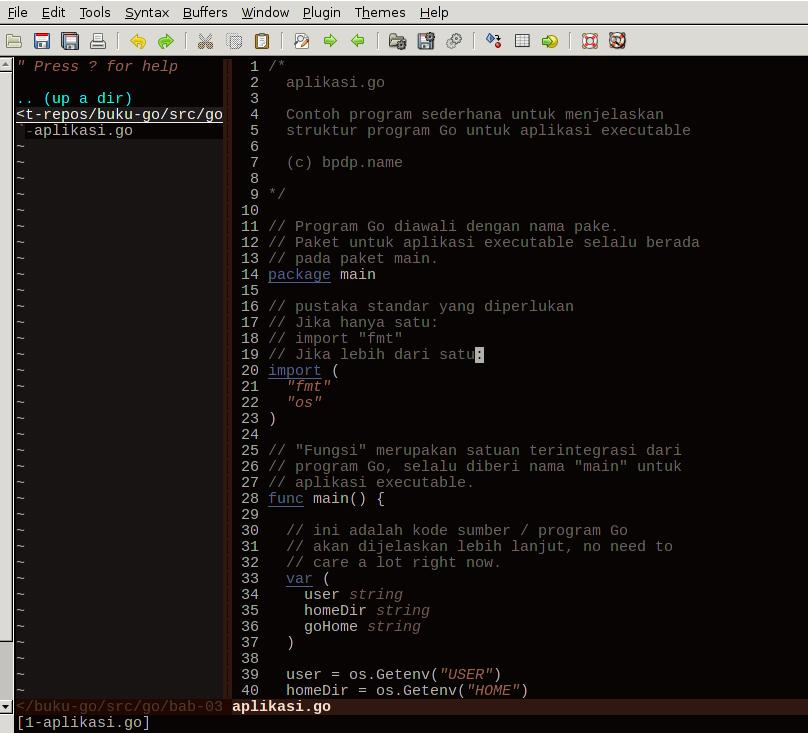
\includegraphics[scale=0.5]{images/vim-go.jpg}
    \end{center}
    \caption{Tampilan gvim untuk mengedit kode sumber Go}
    \label{fig:vim-go}
  \end{figure}


\subsection{Autocompletion}

Vim menyediakan fasilitas \textit{autocompletion} melalui \textit{Omniautocompletion}. Fasilitas ini sudah terinstall saat kita menginstall Vim. Untuk mengaktifkan fasilitas ini untuk keperluan Go, kita harus menginstall dan mengaktifkan Gocode (\url{https://github.com/nsf/gocode}). Sebaiknya kode sumber dari Gocode diambil semua karena ada script Vim yang akan kita gunakan:

\begin{mdframed}[style=catatan]
\begin{verbatim}
$ git clone https://github.com/nsf/gocode.git
Cloning into 'gocode'...
remote: Counting objects: 2491, done.
remote: Compressing objects: 100% (1128/1128), done.
remote: Total 2491 (delta 1323), reused 2449 (delta 1295)
Receiving objects: 100% (2491/2491), 1.07 MiB | 17 KiB/s, done.
Resolving deltas: 100% (1323/1323), done.
$
\end{verbatim}
\end{mdframed}

Setelah itu, install Gocode menggunakan perintah \textbf{go get -u github.com/nsf/gocode}. Hasilnya adalah file \textit{executable binary} \textbf{\$GOROOT/bin/gocode}. Sebelum menggunakan Vim, aktifkan dulu gocode dengan mengeksekusi \textbf{gocode} melalui shell. Setelah itu, tambahkan satu baris di \textbf{\$HOME/.vim/vimrc}: \textbf{set ofu=syntaxcomplete\#Complete} di bawah baris \textbf{filetype plugin indent on}.

Kode sumber lengkap dari \$HOME/.vim/vimrc yang penulis gunakan bisa dilihat pada Listing~\ref{lst:vimrc} adalah sebagai berikut:

\lstset{language=Bash, caption=\$HOME/.vim/vimrc, label={lst:vimrc}}
\lstinputlisting{src/non-go/bab-02/vimrc.txt}

Untuk mengaktifkan completion, kita harus masuk ke mode \textit{Insert} dari Vim, setelah itu tekan \textbf{Ctrl-X, Ctrl-O} secara cepat. Hasil \textit{autocompletion} bisa dilihat di Gambar~\ref{fig:vim-go-completion}.

  \begin{figure}
    \begin{center}
      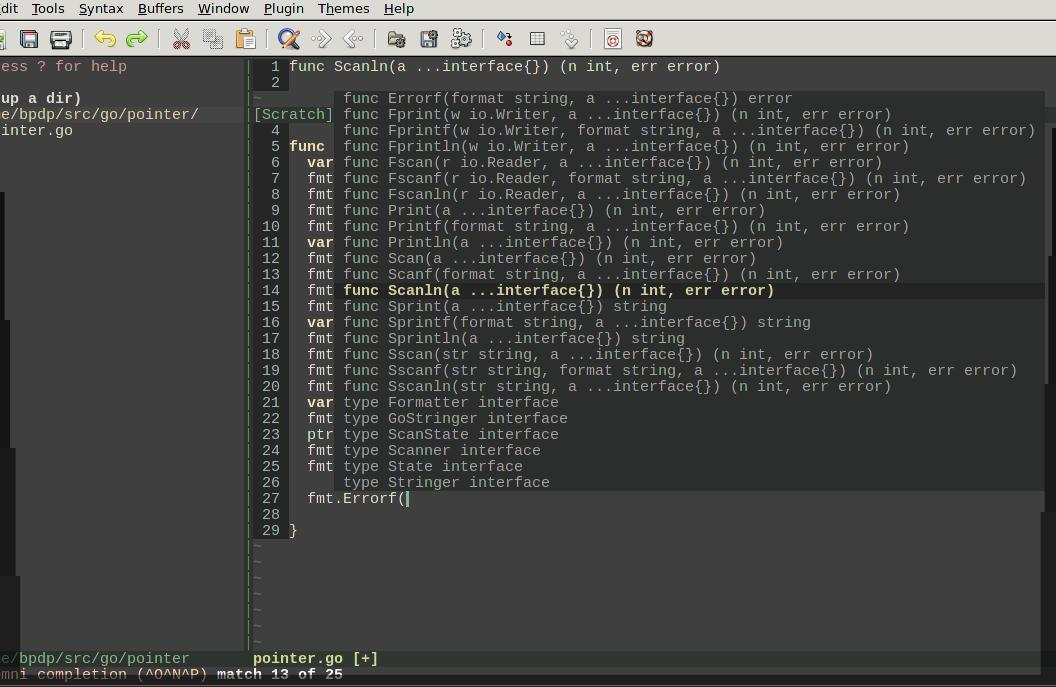
\includegraphics[scale=0.5]{images/vim-go-completion.jpg}
    \end{center}
    \caption{Tampilan gvim untuk mengedit kode sumber Go}
    \label{fig:vim-go-completion}
  \end{figure}

\section{Menggunakan LiteIDE X}

LiteIDE X dibuat oleh visualfc dan tersedia dalam bentuk source code maupun binary. Source code bisa diperoleh di:
\begin{itemize}
  \item \url{http://code.google.com/p/liteide}
  \item \url{https://github.com/visualfc/liteide}
\end{itemize}

Versi binary / installer bisa diperoleh di \url{https://code.google.com/p/golangide/downloads/list}. Jika akan men-download versi binary, ada 2 kategori yang bisa dipilih yaitu LiteIDE X dan LiteIDE X + WebKit. Jenis kedua diperlukan jika kita akan menggunakan HTML Viewer untuk LiteIDE X (biasanya diperlukan jika kita akan membuat aplikasi Web serta memerlukan editor untuk file-file Markdown (.md)).

\subsection{Instalasi}

Instalasi di Linux sangat mudah, hanya tinggal mengekstrak file yang kita download (saat ini versi terakhir adalah versi X18.1) pada suatu direktori dan jika ingin menjalankan cukup dengan mengeksekusi file \$LITEIDEX\_HOME/bin/liteide (cd \$LITEIDEX\_HOME/bin; ./liteide \&):

\section{Software IDE Lain}

Vim dan LiteIDE hanyalah beberapa peranti yang bisa digunakan oleh pengembang. Distribusi Go juga menyediakan dukungan untuk berbagai peranti lunak lain:
\begin{itemize}
  \item \textbf{IntelliJ Idea}. Dukungan untuk Go diwujudkan dalam plugin yang dibuat oleh Mihai Claudiu Toader. Instalasi bisa dilakukan menggunakan menu untuk instalasi plugin dari dalam IntelliJ Idea. Kode sumber untuk plugin ini bisa diperoleh di \url{https://github.com/mtoader/google-go-lang-idea-plugin}
  \item \textbf{Emacs}. Dukungan untuk Go diwujudkan dalam fasilitas \textit{add-on}. Untuk Emacs 24 ke atas, bisa diinstall melalui manajer paket (M-x package-list-packages), cari dan install \textbf{go-mode}. Emacs juga mendukung \textbf{gocode} untuk \textit{completion}.
  \item \textbf{Eclipse}. Dukungan untuk Go diwujudkan melalui plugin \textit{goclipse}, bisa diperoleh di \url{https://code.google.com/p/goclipse/}.
  \item Selain software-software yang telah disebutkan, rata-rata IDE / Editor sudah mempunyai dukungan terhadap bahasa pemrograman Go (JEdit, Sublime-text, Notepad++, dan lain-lain).
\end{itemize}
